\documentclass[11pt, oneside]{article}   	% use "amsart" instead of "article" for AMSLaTeX format
\usepackage{geometry}                		% See geometry.pdf to learn the layout options. There are lots.
\geometry{letterpaper}                   		% ... or a4paper or a5paper or ... 
%\geometry{landscape}                		% Activate for for rotated page geometry
%\usepackage[parfill]{parskip}    		% Activate to begin paragraphs with an empty line rather than an indent
\usepackage{graphicx}				% Use pdf, png, jpg, or eps§ with pdflatex; use eps in DVI mode
								% TeX will automatically convert eps --> pdf in pdflatex		
\usepackage{amssymb,amsmath}
\newcommand{\eqn}[1]{\begin{equation} #1 \end{equation} } 

\newcommand{\dq}[1]{\frac{ d^3 #1}{(2 \pi)^3}}
\newcommand{\bvec}[1]{\boldsymbol{#1} } 
\newcommand{\tdelta}{\tilde{\delta}}
\newcommand{\half}{\frac{1}{2}}
\newcommand{\tdeltaa}{\tilde{\delta}^{(1)} } 
\newcommand{\tdeltab}{\tilde{\delta}^{(2)} } 
\newcommand{\ddirac}{\delta_\rext{D}^3} 
\newcommand{\obs}{\mathcal{O}}


\title{SSC Working Notes }
\author{Joseph E. McEwen}
%\date{}							% Activate to display a given date or no date

\begin{document}
\maketitle


\section{Notations}
We use the following index convention to identify objects:
\begin{itemize}
\item{$\alpha, \beta$ are used for the long-wavelength modes of the density field, i.e. for the super mode $\delta_\alpha$;}
\item{$a, b$ are for the long-wavelength observables, for instance the tangential shear at the survey boundary. These objects are denoted as $\obs_I$;}
\item{$I,J$ are for the short-wavelength observables, for example the power spectrum. These objects are denoted as $\obs_a$; }
\item{$i,j$ are used for the cosmological parameters, $p_i=\{ \Omega_mh^2, \Omega_bh^2, n_s ,...\} $} 
\item{$i_z, j_z$ are used for redshift binning.}
\end{itemize} 
\textbf{I also think it is a good idea that we use the same indexing in the code. For instance, when we create a for loop over redshift bins, we should use $i_z$ as the index in the python code.}
In the code let us try and keep the nomenclature representative of the paper too. For instance we should call $\partial \bar{\delta}/ \partial \delta_\alpha C_{\alpha \beta} \partial \bar{\delta}/ \partial \delta_\beta$= \textbf{sigma2\_SSC} in the code. 

\section{Basic Idea} 
We first define the linear response of a short-wavelength observable to the long-wavelength super modes 
\begin{align} 
\label{lin_response_I}
\obs_I= \bar{\obs}_{I} + \frac{ \partial \obs_I}{\partial \delta_\alpha} \delta_\alpha =\bar{\obs}_{I} + T_{I\alpha} \delta_\alpha ~,
\end{align}
where the  ``bar" designates the observable evaluated with no super modes. We have also defined the transfer function $T_{I\alpha}=\partial \obs_I /\partial \delta_\alpha} $. The covariance matrix is defined by $ C_{IJ} = \langle \obs_I \obs_J \rangle - \langle \obs_I \rangle \langle \obs_J \rangle$.  Using Eq.~ \ref{lin_response_I} the covariance matrix is 
\begin{align}
\label{C_IJ} 
\begin{split}
C_{IJ} &= \bar{C}_{IJ} + T_{I\alpha} \langle \delta_\alpha \delta_\beta \rangle T_{\beta J}  \\
& = \bar{C}_{IJ} + T_{I\alpha} C_{\alpha \beta}  T_{\beta J} ~.
\end{split}
\end{align}
Long-wavelength observables can be used to increase the Fisher information content. We first transform the Fisher information of the long-wavelength observables to the $\alpha-\beta$ basis by
\begin{align} 
F_{\alpha \beta}=\frac{\partial \obs_a}{\partial \delta_\alpha} C_{ab}^{-1} \frac{\partial \obs_b}{\partial \delta_\beta} ~. 
\end{align} 
The information content can be increased by adding Fisher information for each long-wavelength observable 
\begin{align}
F_{\alpha \beta} = F^{(0)}_{\alpha \beta} +  F^{(1)}_{\alpha \beta}+ F^{(2)}_{\alpha \beta} + F^{(3)}_{\alpha \beta}+ ... ~,
\end{align} 
where each matrix $F^{(i)}_{\alpha \beta}$, $i=1,2,3,...$ is constructed from a different long-wavelength observables in the surveys. The 0th Fisher matrix is reserved for $ F^{(0)}_{\alpha \beta} = C_{\alpha \beta}^{-1} = \langle \delta_\alpha \delta_\beta \rangle^{-1}$. By increasing the information content from each long-wavelength observable, we decrease the covariance 
\begin{align} 
C_{\alpha \beta} = \left[ F^{(0)}_{\alpha \beta} +  F^{(1)}_{\alpha \beta}+ F^{(2)}_{\alpha \beta} + F^{(3)}_{\alpha \beta}+ ... \right]^{-1} ~. 
\end{align}
The mitigated covariance is now 
\begin{align} 
C_{IJ}= \bar{C}_{IJ} +  T_{I\alpha}  \left[ F^{(0)}_{\alpha \beta} +  F^{(1)}_{\alpha \beta}+ F^{(2)}_{\alpha \beta} + F^{(3)}_{\alpha \beta}+ ... \right]^{-1} T_{\beta J}   ~.
\end{align} 
The last step in the process is to compute the Fisher information with respect to cosmological parameters 
\begin{align} 
F_{ij}= \frac{\partial \obs_I}{\partial p_i} C_{IJ}^{-1}  \frac{\partial \obs_J}{\partial p_j}~. 
\end{align} 

\section{Code Specific Material}


\subsection{cosmopie module}
The \textbf{cosmopie} module provides cosmology related objects, like the growth factor, distances, and cosmological parameters. This module is usually passed to just about every routine in the code. It is initialized at the beginning and in this way, all objects are referring back to the same cosmology.

\subsection{Halo mass function module}
The \textbf{hmf} module calculates all objects related to the halo mass function. This includes the halo mass function, average number of collapsed objects, the halo bias. Currently this module can only perform the Sheth-Tormen mass function.

\subsection{The basis module}
The basis module takes in the following set of parameters:
\begin{itemize}
\item{$n$ the number of zeros; }
\item{$l_\alpha$ the long wavelength angular mode; }
\item{$R_\text{max}$  the maximum radius of the field (should be larger than the survey depth). 
\end{itemize}
To calculate $\langle \delta_\alpha \delta_\beta \rangle $ the basis module considers $\delta_\alpha$ as a one-dimensional array ordered as $\delta_\alpha[ l_\alpha, m_\alpha, n]$, so that the first entries corresponds to $[0,0,0], ...,[0,0,n],[1,-1,1],..,[1,-1,n],[1,0,0],...$ (\textbf{it should be verified that this is the right ordering in the code}).This will be called $\alpha$ ordering. The covariance is ordered in the same way $[l_\alpha, m_\alpha, n] \times [l_\beta, m_\beta, n]$. 

The basis module contains objects:
\begin{itemize}
\item{\textbf{Get\_C\_alpha\_beta} returns $C_{\alpha \beta}^{(0)}$, the covariance matrix composed of the long wavelength modes;}
\item{ \textbf{Get\_F\_alpha\_beta} returns $F_{\alpha \beta}^{(0)}$, the Fisher matrix constructed from the long wavelength modes;}
\item{ \textbf{ddelta\_bar\_ddelta\_alpha} a function that returns $\partial \bar{\delta}/\partial \delta_\alpha$ given a region of the universe. }
\end{itemize} 

\subsection{The short wavelength array}
The $\mathcal{O}_I$ array is ordered as $[x, z_{\text{avg},i_z}]$, where $x$ is any of the following $k,l,\{k,\mu\}$, and this is called $I$ ordering. The covariance matrix built from $\mathcal{O}_I$ follows the same ordering. 

\subsection{The long wavelength array}
The $\mathcal{O}_a$ array is ordered as $[x, z_{\text{avg},i_z}]$, where $x$ is any of the following $k,l,\{k,\mu\}$, and this is called $a$ ordering. The covariance matrix built from $\mathcal{O}_a$ follows the same ordering. However, all functions that relate to  $\mathcal{O}_a$  build the matrix $F_{\alpha \beta} = \frac{\partial \mathcal{O}_a}{\partial \delta_\alpha} C_{ab}^{-1}  \frac{\partial \mathcal{O}_b}{\partial \delta_\beta}$, which is $\alpha$ ordered. 

\subsection{Increased Fisher Matrix}
The function \textbf{Get\_SSC\_covar} builds the covariance matrix $C_{IJ}= \bar{C}_{IJ} + T_{I\alpha} C_{\alpha \beta} T_{J\beta}$. This matrix is $I$ ordered. 
The first routine that \textbf{Get\_SSC\_covar} should build is the Fisher matrices for each long wavelength observable. Each Fisher matrix should then be added and this value should be stored as this should be stored as the object \textbf{F\_alpha\_beta}. The inverse of \textbf{F\_alpha\_beta} is then taken and this object is stored as \textbf{C\_alpha\_beta}. Then for each short wavelength observable $\frac{\partial \bar{\delta}}{\partial \delta_\alpha} C_{\alpha \beta} \frac{\partial \bar{\delta}}{\partial \delta_\beta}$ is calculated. This object is stored as \textbf{sigma2\_SSC}. The final object calculated is 
$\frac{\partial \obs_I}{\partial \bar{\delta}} \frac{\partial \bar{\delta}}{\partial \delta_\alpha} C_{\alpha \beta} \frac{\partial \bar{\delta}}{\partial \delta_\beta} \frac{\partial \obs_I}{\partial \bar{\delta}}$. This object is stored as \textbf{C\_SSC\_IJ}. 

\subsection{Response of power spectrum to background density} 
The following relations are used to calculate $ d P(k)/d\bar{\delta}$ for $P(k)$ computed linearly, in standard perturbation theory, and using halo fit. These routines are calculated in the python model \textbf{power\_response.py}. \textbf{We still need to include the form for the HOD power spectrum.} 
\begin{itemize} 
\item{linear 
\begin{align} 
\frac{ d \log P(k)}{d \bar{\delta}}=\frac{68}{21} - \frac{1}{3} \frac{ d \log k^3 P(k)}{d \log k}~, 
\end{align} 
} 
\item{1-loop perturbation theory
\begin{align} 
\frac{ d \log P(k)}{d \bar{\delta}}=\frac{68}{21} - \frac{1}{3} \frac{ d \log k^3 P(k)}{d \log k} + \frac{26}{21} \frac{P_{22}(k) + P_{13}(k)}{P(k)} ~, 
\end{align} 
} 
\item{halo fit power spectrum
\begin{align} 
\frac{ d \log P(k)}{d \bar{\delta}}= \frac{13}{21} \frac{ d \log P(k)}{d \log \sigma_8} + 2 - \frac{1}{3} \frac{ d \log k^3 P(k)}{d \log k}~, 
\end{align} 
}
\end{itemize} 

\section{Importance of Super Sample Covariance} 
%\documentclass[11pt, oneside]{article}   	% use "amsart" instead of "article" for AMSLaTeX format
%\usepackage{geometry}                		% See geometry.pdf to learn the layout options. There are lots.
%\geometry{letterpaper}                   		% ... or a4paper or a5paper or ... 
%\geometry{landscape}                		% Activate for for rotated page geometry
%\usepackage[parfill]{parskip}    		% Activate to begin paragraphs with an empty line rather than an indent
%\usepackage{graphicx}				% Use pdf, png, jpg, or eps§ with pdflatex; use eps in DVI mode
%								% TeX will automatically convert eps --> pdf in pdflatex		
%\usepackage{amssymb,amsmath}
\newcommand{\sph}[2]{Y^\text{R}_{l_#1 m_#1}(\hat{#2})}

\newcommand{\jl}[1]{j_{l_#1}}
\newcommand{\dk}{\frac{ d^3 \mathbf{k}}{(2 \pi)^3}} 
\newcommand{ \dkv}[1]{\frac{ d^3 \mathbf{k}_{#1}}{(2 \pi)^3}} 
\newcommand{\obs}{\mathcal{O}}

\subsection{Super Sample Covariance in the Literature}

Who been playing SSC? 

\cite{2013PhRvD..87l3504T} showed that the sample variance of the power spectrum is dominated by modes larger than the survey region. They also showed that halo sample variance and super sample covariance are related by the squeezed configurations of the trispectrum. Fig.~3 of their paper shows that the diagonal non-Gaussian covariance in the power spectrum is dominated by the SSC effect, for $k > 1 ~h/$Mpc the SSC is up to two orders of magnitude larger than the trispectrum contribution. 

\cite{2014PhRvD..89h3519L} compared the direct quantification of the SSC effect on the covariance of the power spectrum generated in subvolumes of large simulation to the SSC model of the power spectrum response to the background mode. Fig.~6 of their paper shows that the diagonal non Gaussian covariance in from the sub does matches the SSC model + small boxes, where small boxes are computed with periodic boundary conditions (i.e. they have no SSC-periodic boundary conditions can not capture SSC effects). 

\cite{2016PhRvD..93f3507L} compared the bias computed from the halo mass function in separate universe simulations with the bias computed from ratios of correlation functions. Fig.~4 and 5 of their paper show that the average bias and bias computed from the response of the halo mass function compared to the bias computed from correlations functions is in well agreement. They find 1-2 \% for average bias in the 1 to 4 range and 4-5\% agreement for the average bias at bias value of 8. There work provides a consistency between a one-point functions (the halo mass functions), and two-point functions (the halo-mass functions and mass-mass functions). 

\section{Theory}
%\documentclass[11pt, oneside]{article}   	% use "amsart" instead of "article" for AMSLaTeX format
%\usepackage{geometry}                		% See geometry.pdf to learn the layout options. There are lots.
%\geometry{letterpaper}                   		% ... or a4paper or a5paper or ... 
%\geometry{landscape}                		% Activate for for rotated page geometry
%\usepackage[parfill]{parskip}    		% Activate to begin paragraphs with an empty line rather than an indent
%\usepackage{graphicx}				% Use pdf, png, jpg, or eps§ with pdflatex; use eps in DVI mode
%								% TeX will automatically convert eps --> pdf in pdflatex		
%\usepackage{amssymb,amsmath}
\newcommand{\sph}[2]{Y^\text{R}_{l_#1 m_#1}(\hat{#2})}

\newcommand{\jl}[1]{j_{l_#1}}
\newcommand{\dk}{\frac{ d^3 \mathbf{k}}{(2 \pi)^3}} 
\newcommand{ \dkv}[1]{\frac{ d^3 \mathbf{k}_{#1}}{(2 \pi)^3}} 
\newcommand{\obs}{\mathcal{O}}

\subsection{Trispectrum Consistency Relation}

The trispectrum is defined as
\begin{align} 
\langel \delta(\mathbf{k}_1) \delta(\mathbf{k}_2)\delta(\mathbf{k}_3)\delta(\mathbf{k}_4) \rangle = (2 \pi)^3 \delta_\text{D}(\mathbf{k}_1+ \mathbf{k}_2+ \mathbf{k}_3+ \mathbf{k}_4 )T(\mathbf{k}_1, \mathbf{k}_2, \mathbf{k}_3, \mathbf{k}_4 )~. 
\end{align} 

\begin{align}
\begin{split} 
T(\mathbf{k}_1, \mathbf{q}-\mathbf{k}_1, \mathbf{k}_2, \mathbf{q}- \mathbf{k}_2) & = \\
\end{split} 
\end{align} 

\documentclass[11pt, oneside]{article}   	% use "amsart" instead of "article" for AMSLaTeX format
\usepackage{geometry}                		% See geometry.pdf to learn the layout options. There are lots.
\geometry{letterpaper}                   		% ... or a4paper or a5paper or ... 
%\geometry{landscape}                		% Activate for for rotated page geometry
%\usepackage[parfill]{parskip}    		% Activate to begin paragraphs with an empty line rather than an indent
\usepackage{graphicx}				% Use pdf, png, jpg, or eps§ with pdflatex; use eps in DVI mode
								% TeX will automatically convert eps --> pdf in pdflatex		
\usepackage{amssymb,amsmath}


\newcommand{\sph}[2]{Y^\text{R}_{l_#1 m_#1}(\hat{#2})}

\newcommand{\jl}[1]{j_{l_#1}}
\newcommand{\dk}{\frac{ d^3 \mathbf{k}}{(2 \pi)^3}} 
\newcommand{ \dkv}[1]{\frac{ d^3 \mathbf{k}_{#1}}{(2 \pi)^3}} 
\newcommand{\obs}{\mathcal{O}}

\title{The $\delta_\alpha$ basis and covariance $\langle \delta_\alpha \delta_\beta \rangle$}
\author{Joseph E. McEwen}
%\date{}							% Activate to display a given date or no date

\begin{document}
\maketitle

\section{Spherical basis functions}
For spherical geometry we use the following basis, composed of the spherical Bessel function and spherical harmonic:
\begin{align} 
\psi_\alpha(r, \theta, \phi) = j_{l_\alpha}(k_\alpha r) Y^\text{R}_{l_\alpha m_\alpha}(\theta, \phi) ~, 
\end{align} 
where $Y^\text{R}_{lm}(\theta, \phi) $ is the real spherical harmonic. The real spherical harmonics are defined as 

\begin{align}\label{real_harmonic1}
Y^\text{R}_{lm} \equiv
\begin{cases} \frac{i}{\sqrt{2}} \left( Y_{l}^m  - (-1)^{-m} Y_{l}^m \right)& \text{if }  m < 0 \\
Y_{l0} & \text{if } m=0 \\
\frac{1}{\sqrt{2}}\left( Y_{l}^{-m} + (-1)^mY_{l}^m\right) & \text{if } m > 0 ~,
\end{cases}
\end{align} 
%\begin{align}
%Y^\text{R}_{lm} =
%\begin{cases} \frac{i}{\sqrt{2}} \left( Y_{lm}  - (-1)^m Y_{l-1m} \right)& \text{if }  m < 0 \\
%Y_{l0} & \text{if } m=0 \\
%\frac{1}{\sqrt{2}}\left( Y_{l-m} + (-1)^mY_{lm}\right) & \text{if } m > 0 ~.
%\end{cases}
%\end{align} 
We write a super survey mode as 
\begin{align}
\delta_\alpha(k_\alpha)& = \int \delta(\mathbf{r}) \jl{\alpha}(k_\alpha r) \sph{\alpha}{r} d^3 \mathbf{r}~. 
\end{align}

\section{Mean background density in a region}
The mean background density in a region is composed of the super modes:

\begin{align}
\label{bar_delta}
\bar{\delta}= \displaystyle \sum_\alpha \frac{3}{r_\text{max}^3 - r_\text{min}^3} \int_{r_\text{min}}^ {r_\text{max} }dr ~ r^2 j_{l_\alpha}(k_\alpha r) \delta_\alpha(k_\alpha) \frac{1}{2\sqrt{\pi} a_{00}} \underbrace{ \int_{\theta_1}^{\theta_2 }\int_{\phi_1}^{\phi_2} d  \theta d \phi ~\sin(\theta)\sph{\alpha}{r}}_{a_{l_\alpha m_\alpha}} ~.
\end{align}


In practice we are interested in derivatives of observables with respect to the $\delta_\alpha$. This is accomplished by chain rule 
\begin{align}
\frac{\partial f}{\partial \delta_\alpha}= \frac{\partial f}{\partial \bar{\delta}} \frac{\partial \bar{\delta}}{\partial \delta_\alpha}~.
\end{align} 
The derivative is computed from Eqn.~\ref{bar_delta}
\begin{align}
\frac{\partial \bar{\delta} }{ \partial \delta_\alpha}=
\frac{3 N_\alpha}{r_\text{max}^3 - r_\text{min}^3} \int_{r_\text{max}}^ {r_\text{min} }dr ~ r^2 j_{l_\alpha}(k_\alpha r)  \frac{1}{2\sqrt{\pi} a_{00}}  \int_{\theta_1}^{\theta_2 } \int_{\phi_1}^{\phi_2} d\theta d \phi ~\sin(\theta)\sph{\alpha}{r}~,
\end{align}

where $N_\alpha$ is defined in \eqref{normalization}.

 
\section{Covariance of super modes}
In our basis the super survey mode is defined as 
\begin{align} 
\begin{split} 
\delta_\alpha(k_\alpha)& = \int \delta(\mathbf{r}) \jl{\alpha}(k_\alpha r) \sph{\alpha}{r} d^3 \mathbf{r}  \\
& = \int \dk \delta(\mathbf{k}) \int_0^{r_\text{max}} dr^2 \jl{\alpha}(k_\alpha r) \int d^2 \hat{r} e^{ikr \hat{k} \cdot \hat{r}} \sph{\alpha}{r} \\
& =4 \pi i^{l_\alpha}\int  \dk \delta(\mathbf{k})  \sph{\alpha}{k}  \int_0^{r_\text{max}} dr^2 \jl{\alpha}(k_\alpha r) \jl{\alpha}(kr)  ~,
\end{split} 
\end{align} 
where in the second equality $\delta(\mathbf{r})=(2\pi)^{-3} \int d^3 \mathbf{k} \exp(i \mathbf{k} \cdot \mathbf{r}) \delta(\mathbf{k})$ was used and in the third equality the following identity was used 
\begin{align} \int_{S^2} d^2 \hat{r} \sph{\alpha}{r} e^{i \mathbf{k} \cdot \mathbf{r}} = 4 \pi i^{l_\alpha} j_{l_\alpha}(k r)\sph{\alpha}{k}~.
\end{align}
Including a normalization
\begin{align}\label{normalization}
N_\alpha&=\int{d^3\mathbf{r}\sph{\alpha}{r} \sph{\alpha}{r} j_\alpha(k_\alpha r) j_\alpha(k_\alpha r)} \\
&=  I_\alpha(k_\alpha, r_{\text{max}})  \int_\Omega \sph{\alpha}{r} \sph{\alpha}{r} \hat{r}\\
& =I_\alpha(k_\alpha, r_{\text{max}})  
\end{align}
where $ I_\alpha(k_\alpha, r_{\text{max}}) $ is as defined in \eqref{norm_final} and $ \int_\Omega \sph{\alpha}{r} \sph{\alpha}{r} \hat{r}=1$, we have
\begin{align} 
\delta_\alpha= \frac{4 \pi i^{l_\alpha}}{N_\alpha} \int  \dk \delta(\mathbf{k})  \sph{\alpha}{k}  \int_0^{r_\text{max}} dr^2 \jl{\alpha}(k_\alpha r) \jl{\alpha}(kr)  ~.
\end{align} 
To get the covariance of the super survey field we take the ensemble average:
\begin{align} 
\begin{split} 
\langle \delta_\alpha \delta_\beta \rangle &= \frac{ (4 \pi)^2}{N_\alpha N_\beta} \int  \dkv{1} \dkv{2} \langle \delta(\mathbf{k}_1) \delta^*(\mathbf{k}_2) \rangle \sph{\alpha}{k_1} \sph{\beta}{k_2} \\
& \;\;\; \times   \int_0^{r_\text{max}}  dr r^2 \jl{\alpha}(k_\alpha r) \jl{\alpha}( k_1 r) \int_0^{r_\text{max}}  dr r^2 \jl{\beta}(k_\beta r) \jl{\beta}( k_2 r)  \\
&= \frac{ (4 \pi)^2}{N_\alpha N_\beta} \int \dk P(k) I_\alpha(k, r_\text{max}) \times I_\beta(k, r_\text{max})\sph{\alpha}{k_1}Y^R_{l_\beta m_\beta}(-\hat{k_1})\\
&=\frac{2}{\pi N_\alpha N_\beta}\int{k^2 dk P(k)(-1)^{l_\beta} \delta_{l_\alpha,l_\beta}\delta_{m_\alpha,m_\beta} I_\alpha(k, r_\text{max}) \times I_\beta(k, r_\text{max})}~,
\end{split} 
\end{align} 
where $(2 \pi)^3 \delta^3_\text{D}( \mathbf{k} + \mathbf{k}') P(k) =  \langle \delta(\mathbf{k}) \delta^*(\mathbf{k}') \rangle$ was used along with the definition 
\begin{align}\label{i_alpha}
\begin{split} 
I_\alpha(k,  r_\text{max}) & =  \int_0^{r_\text{max}}dr r^2 \jl{\alpha}(k_\alpha r) \jl{\alpha}( k r) \\
& = \frac{\pi}{2} \sqrt{ \frac{1}{k _ \alpha k}} \int_0^{r_\text{max}}dr r J_{l_\alpha+ 1/2}(k_\alpha r)  J_{l_\alpha+ 1/2}( k r) \\
& = \frac{\pi}{2} \frac{ r_\text{max}}{ \sqrt{ k _ \alpha k}}\frac{\left[k_\alpha J_{l_\alpha+ 1/2}( k  r_\text{max})J_{l_\alpha+ 1/2}'(k_\alpha  r_\text{max}) - k J_{l_\alpha+ 1/2}(k_\alpha  r_\text{max})J_{l_\alpha+ 1/2}'(k  r_\text{max})\right]}{k^2 - k_\alpha^2}\\
& = \frac{\pi}{2} \frac{ r_\text{max}}{ \sqrt{ k _ \alpha k}}\frac{\left[k_\alpha J_{l_\alpha+ 1/2}( k  r_\text{max})J_{l_\alpha- 1/2}(k_\alpha  r_\text{max}) - k J_{l_\alpha+ 1/2}(k_\alpha  r_\text{max})J_{l_\alpha- 1/2}(k  r_\text{max})\right]}{k^2 - k_\alpha^2}\\
& = \frac{\pi}{2} \frac{ r_\text{max}}{ \sqrt{ k _ \alpha k}}\frac{k_\alpha J_{l_\alpha+ 1/2}( k  r_{\text{max}})J_{l_\alpha- 1/2}(k_\alpha  r_\text{max})}{k^2 - k_\alpha^2}~,
\end{split} 
\end{align}

where in the last step we have use $J_{l_\alpha+1/2}(k_\alpha r_max)=0$, from the defining property of $k_\alpha$. In the special case $k=k_\alpha$, we can simplify $N_\alpha = I_\alpha(k,r_max)$:

\begin{align}
N_\alpha = I_\alpha(k_\alpha,  r_\text{max}) & = \lim_{k\to k_\alpha} \frac{\pi}{2} \frac{ r_\text{max}}{ \sqrt{ k _ \alpha k}}\frac{k_\alpha J_{l_\alpha+ 1/2}( k  r_\text{max})J_{l_\alpha- 1/2}(k_\alpha  r_\text{max})}{k^2 - k_\alpha^2}\\
&=\lim_{k\to k_\alpha}\frac{\pi r_\text{max}}{2} \frac{J_{l_\alpha+ 1/2}( r_\text{max})J_{l_\alpha- 1/2}(k_\alpha  r_\text{max})}{k^2 - k_\alpha^2}\label{pre_lhopital}\\
&=\lim_{k\to k_\alpha}\frac{\pi r_\text{max}}{2} \frac{r_\text{max}J'_{l_\alpha+ 1/2}(k r_\text{max})J_{l_\alpha- 1/2}(k_\alpha  r_\text{max})}{2 k}\label{post_lhopital}\\
&=\lim_{k\to k_\alpha}\frac{\pi r_\text{max}^2}{2} \frac{\left[\frac{l_\alpha+1/2}{k r_{\text{max}}}J_{l_\alpha+1/2}(k r_\text{max})-J_{l_\alpha+3/2}(k_\alpha{r_max})\right]J_{l_\alpha- 1/2}(k_\alpha  r_\text{max})}{2 k}\label{post_recurrence}\\
&=-\frac{\pi r_\text{max}^2}{4 k_\alpha}J_{l_\alpha+3/2}(k_\alpha{r_\text{max}})J_{l_\alpha- 1/2}(k_\alpha  r_\text{max})\label{norm_final}
\end{align}

Where between \eqref{pre_lhopital} and \eqref{post_lhopital} we have used L'H$\hat{\text{o}}$pital's rule, and between \eqref{post_lhopital} and \eqref{post_recurrence} we have used a recurrence relation for the Bessel functions, $J'_n(x)=\frac{n}{x}J_n{x}-J_{n+1}(x)$.
\section{The computation of basis objects}
The radial basis function should be zero at the sector boundary. Thus, fiven the maximum radius of the sector $r_\text{max}$ the super wave vector $k_\alpha$ is found by 
\begin{align}
 j_{l_\alpha}(k_\alpha r_\text{max})=0.
 \end{align}

%\section{How to obtain derivatives by finite differences}
%We need to calculate objects like $\partial \obs_I/ \partial \delta_\alpha$. This is done by applying the chain rule. 
%
%\begin{align} 
%\frac{\partial \obs_I}{ \partial \delta_\alpha} = \frac{\partial \obs_I}{ \partial \Theta^i} \frac{\partial \Theta^i}{\partial \bar{\delta} } \frac{\partial \bar{\delta}}{\delta_\alpha} ~. 
%\end{align}
%When the observable is to complicated that an analytic method for the derivative is not possible, or is too cumbersome to attempt, we can use a finite difference approach. We can take $\bar{\delta}=\pm \epsilon$. As long as $\epsilon$ is small we should be in the linear regime (which is the region we are limiting our analysis too). Then we can take 
%
%\begin{align}
% \frac{\partial \obs_I}{ \partial \Theta^i} = \frac{ \obs_I(+ \epsilon) - \obs_I(- \epsilon)}{2\delta\Theta^I( \epsilon)} ~,
% \end{align} 
%and in the above $  \obs_I(+ \epsilon)$ means that the observable is calculated in the separate universe approch, where $\bar{\delta}=\pm\epsilon$ corresponds to a change in cosmological parameters.  The figure below illustrates this approach. The point being, is that we can choose $\epsilon$ arbitrarily (as long as we are in the linear regime) and we will still get the correct derivative, because it is just a slope. 
% 
% \begin{figure}[h]
%  \caption{Finite difference approach.}
%  \centering
%    \includegraphics[width=\textwidth]{finite_diff_O.pdf}
%\end{figure}

\end{document}  
%\documentclass[a4paper,11pt]{article}
%%\documentclass[11pt, oneside]{article} 
%% MNRAS is set in Times font. If you don't have this installed (most LaTeX
%% installations will be fine) or prefer the old Computer Modern fonts, comment
%% out the following line
%%\usepackage{txfonts}
%%\usepackage{newtxtext,newtxmath}
%% Depending on your LaTeX fonts installation, you might get better results with one of these:
%%\usepackage{mathptmx}
%%\usepackage{txfonts}
%
%% Use vector fonts, so it zooms properly in on-screen viewing software
%% Don't change these lines unless you know what you are doing
%\usepackage[T1]{fontenc}
%\usepackage{ae,aecompl}
%\usepackage[caption=false,font=footnotesize]{subfig}
%\usepackage{natbib}
%
%
%%%%%% AUTHORS - PLACE YOUR OWN PACKAGES HERE %%%%%
%
%% Only include extra packages if you really need them. Common packages are:
%\usepackage{graphicx}	% Including figure files
%\usepackage{amsmath}	% Advanced maths commands
%\usepackage{amssymb}	% Extra maths symbols
%
%
%
%\def\lesssim{\mathrel{\hbox{\rlap{\hbox{\lower5pt\hbox{$\sim$}}}\hbox{$<$}}}}
%\def\gtrsim{\mathrel{\hbox{\rlap{\hbox{\lower5pt\hbox{$\sim$}}}\hbox{$>$}}}}
%\def\mnras{MNRAS}
%\def\apj{ApJ}
%\def\apjl{ApJL}
%\def\aj{AJ}
%\def\planss{Planet.~Space Sci.}
%\def\prd{Phys.~Rev.~D}
%\def\apjs{ApJS}
%\def\aap{A\&A}
%\def\nat{Nature}
%\def\apss{Ap\&SS}
%\def\lcdm{$\Lambda$CDM }
%\def\hMpc{h^{-1} \text{Mpc}}
%\def\rgm{r_{\rm gm}}
%\def\hMsun{h^{-1}M_\odot}
%
%\def\xigg{\xi_{\rm gg}}
%\def\xigm{\xi_{\rm gm}}
%\def\ximm{\xi_{\rm mm}}
%\def\Omegam{\Omega_{\rm m}}
%\def\kms{\text{kms}^{-1}}
%
%\newcommand{\ef}[2]{e^{#1}_{\phantom{p}#2}}
%\newcommand{\einv}[2]{e_{#1}^{\phantom{p}#2}}
%
%
%%\voffset=-0.69in
%%\hoffset=0.12in
%

\section{Separate Universe Approach}

\subsection{Fermi Normal Coordinates}
Here I would like to reserve the separate universe equations. It will be similar to Baldauf. 


Fermi normal coordinate reference include Chp.~ 13 of \cite{misner1973gravitation}, Chp.~1 of \cite{poisson2004relativist} the \cite{manasse1963fermi}
Transport the tetrad $e^a_{\;A}$ along the geodesic $\gamma$, such that  $e^a_{\;\;0}=u^{a}(\tau)$, where $\mathbf{u}=d\gamma/d\tau$. And
\begin{align} 
g_{ab} e^a_{\;\;A}e^b_{\;\;B}= \eta_{AB} ~.
\end{align} 

\begin{align} 
\grad_\mathbf{u} e_A= u^a\nabla_a e^b_{\;\; A} = - u^a \Omega_c^{\;\; b} e^c_{\;\; A}~, 
\end{align} 
where $\Omega^{ab}=a^au^b - a^bu^a + u_c\omega_d \epsilon^{cdab}$. In the absence of acceleration and rotations the above equation gives 
\begin{align} 
 u^a\nabla_a e^b_{\;\; A}=0~.
 \end{align} 

\subsection{Power Spectrum Response}  

\begin{figure}[!ht]
 \centering
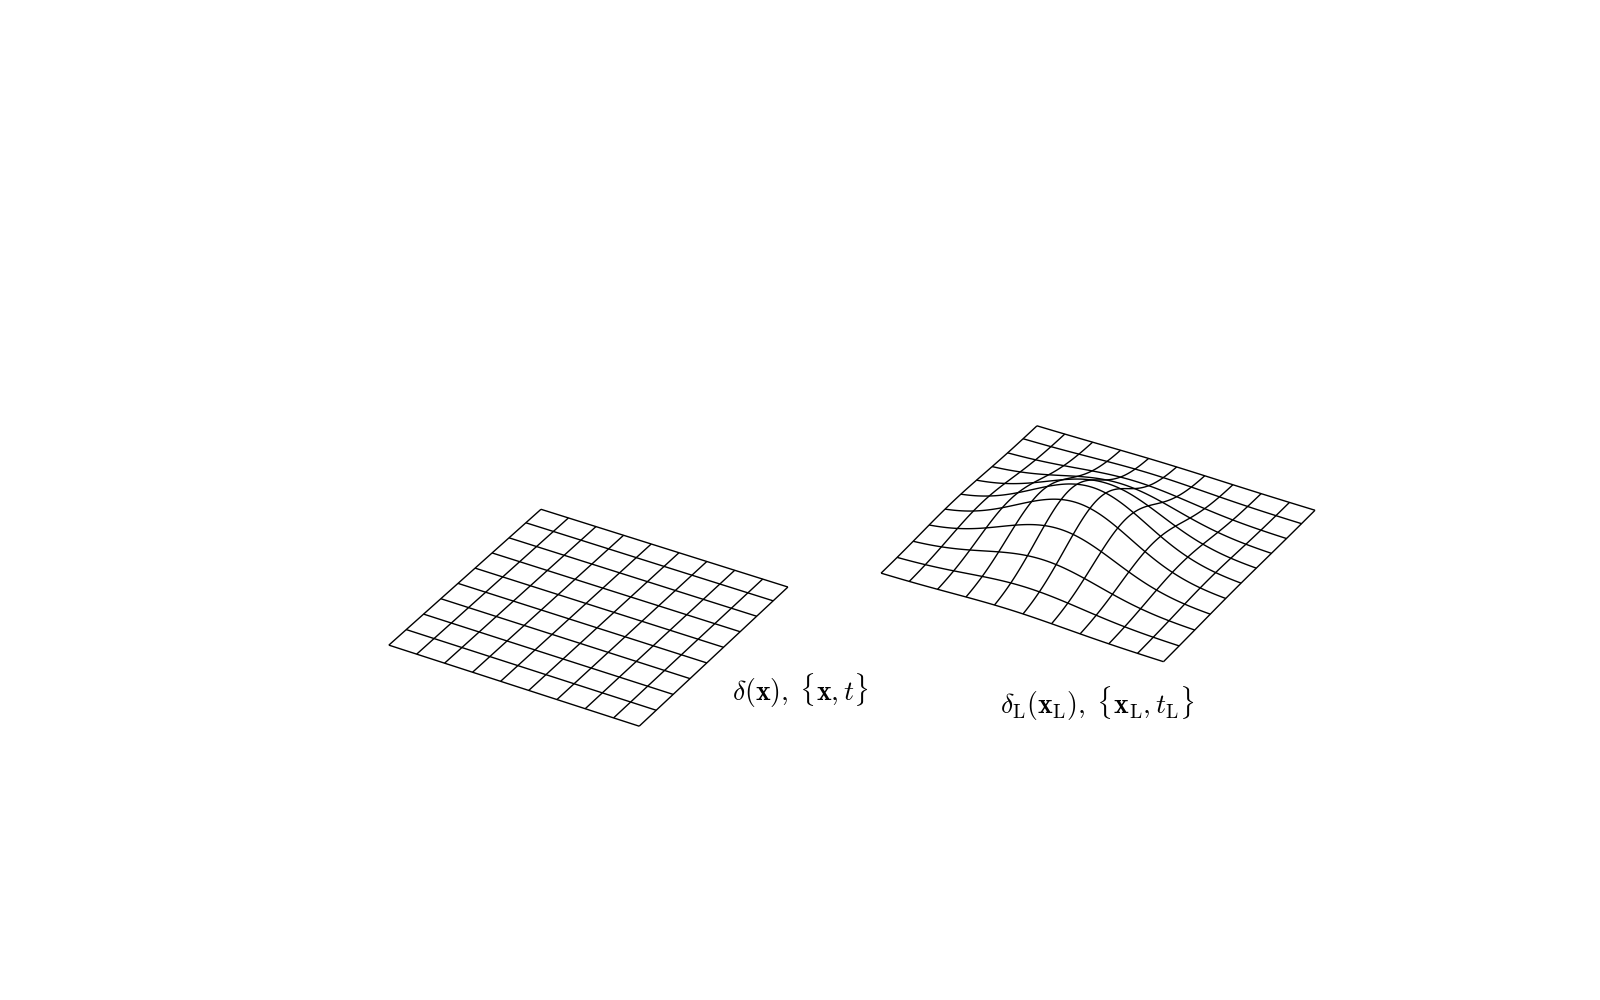
\includegraphics[width=1\textwidth]{manifolds.png}
  \caption{Illustration of the difference in correlations functions. The difference in any correlation (in real or Fourier space) is defined as difference in correlates on two different manifolds. The computation requires the appropriate mapping between manifolds. }
\label{fig:manifolds}
\end{figure}

The response of correlation function to a $\bar{\delta}$ is computed by 
\begin{align} 
\label{corr_response}
\frac{d \xi(r,t)}{d \bar{\delta}}= \frac{ \Phi[ \xi_\text{L}(r_\text{L},t_\text{L})]- \xi(r)}{\bar{\delta} } ~,
\end{align} 
where $\Phi$ is the mapping from the L universe to the ``standard" universe. The mapping is as follows 
 \begin{align} 
\begin{split} 
\xi_\text{L}(r_\text{L}, t_\text{L}) &= \langle \delta_\text{L} | \delta_\text{L} \rangle_{r_\text{L},t_\text{L}} \\
& =  \langle \delta (1+ \bar{\delta} ) + 1 | \delta(1+ \bar{\delta} ) + 1  \rangle_{r + \bar{\delta}/3,t_\text{L}} \\
& = \langle \delta | \delta \rangle_{r + \bar{\delta}/3,t_\text{L}} + 2 \bar{\delta} \langle \delta | \delta \rangle_{r + \bar{\delta}/3,t_\text{L} }+ \mathcal{O}(\bar{\delta}^2) \\
& = \xi(r + \bar{\delta}/3,t_\text{L}) + 2 \bar{\delta}\xi(r + \bar{\delta}/3,t_\text{L})  \\
& = \xi(r, t_\text{L}) + \frac{ \bar{\delta} }{3}r \partial_r \xi(r,t_\text{L}) + 2 \bar{\delta} \xi(r, t) + \mathcal{O}(\bar{\delta}^2) ~.
\end{split} 
\end{align} 
where the subscripts in the first few lines represent the position and time arguments. Plugging back into Eqn.~\ref{corr_response} gives 
\begin{align}  
\frac{d \xi(r,t)}{d \bar{\delta}} =\frac{ \xi(r, t_\text{L}) + \frac{ \bar{\delta} }{3}r \partial_r \xi(r,t_\text{L}) + 2 \bar{\delta} \xi(r, t) - \xi(r,t)}{\bar{\delta}} ~. 
\end{align} 
I have not transformed the time coordinate. I will do this later. For the linear and SPT power spectrum, the time coordinate transformation will correspond to change in the growth factor. 
The derivative term in Fourier space is computed as follows:
\begin{align} 
\begin{split} 
r \partial_r \xi(r) & =r\hat{r} \cdot \mathbf{\nabla} \xi(r) = \hat{r} \cdot  \mathbf{\nabla}  \int \frac{d^3 \mathbf{k}}{(2 \pi)^3} e^{i \mathbf{k} \cdot \mathbf{r} } P(k) \\
& = r\hat{r} \cdot \int \frac{d^3 \mathbf{k}}{(2 \pi)^3} ~i \mathbf{k}~ e^{i \mathbf{k} \cdot \mathbf{r} } P(k) \\
& = \int \frac{d^3 \mathbf{k}}{(2 \pi)^3} ~i \mathbf{r}~ e^{i \mathbf{k} \cdot \mathbf{r} } \cdot \mathbf{k}P(k) \\
& = \int \frac{d^3 \mathbf{k}}{(2 \pi)^3} ~\mathbf{\nabla}_\mathbf{k}~ e^{i \mathbf{k} \cdot \mathbf{r} } \cdot \mathbf{k}P(k) \\
& =- \int \frac{d^3 \mathbf{k}}{(2 \pi)^3} e^{i \mathbf{k} \cdot \mathbf{r} }   ~\mathbf{\nabla}_\mathbf{k}~\cdot [\mathbf{k}P(k) ]\\
& =- \int \frac{d^3 \mathbf{k}}{(2 \pi)^3} e^{i \mathbf{k} \cdot \mathbf{r} }  [ 3 P(k) + k \frac{d P(k)}{d k}] ~.
\end{split} 
\end{align} 
Therefore the power spectrum response is 
\begin{align} 
\frac{ d P(k)}{d \bar{\delta}}=  \frac{1}{\bar{\delta} }\left[ P(k,t_\text{L}) - \frac{\bar{\delta}}{3} [ 3P(k,t_\text{L} )+ k \frac{d P(k)}{dk}] + 2 \bar{\delta} P(k, t_\text{L}) - P(k,t)\right] ~. 
\end{align} 

\subsection{Linear power spectrum response} 
Linear growth factors in the L universe compared to the ``standard" universe are 
\begin{align} 
G_\text{L}( a[ 1 - \frac{1}{3} \bar{\delta} ]) = G(a)\left[ 1 + \frac{13}{21} \bar{\delta} \right]~. 
\end{align} 

To relate the linear power spectrum at time $t_\text{L}$ to time $t$ requires the ratio of growth factors squared and we have 
\begin{align} 
P_\text{lin}(k, t_\text{L})= \left[ 1 + \frac{26}{21} \bar{\delta}\right] P(k, t) 
\end{align} 

Plugging the above back into the master equation for power spectrum response gives 
\begin{align}
\frac{ d P(k)}{d \bar{\delta}} = \frac{68}{21} P(k) - \frac{1}{3} [ 3 P(k) + k \frac{d P(k)}{dk} ] ~. 
\end{align} 

\subsection{1 -loop perturbation theory}
The 1-loop growth factor relation is 
\begin{align}
P_{1-loop}(k,z)= G^2 P_{11}(k) + G^4 [P_{22}(k) + P_{13}(k)] ~, 
\end{align} 
So the transformation is 
\begin{align} 
P_{1-loop}(k,t_\text{L})=  \left[ 1 + \frac{26}{21} \bar{\delta}\right] P_{11}(k,t) +  \left[ 1 + \frac{52}{21} \bar{\delta}\right] [ P_{22}(k,t) + P_{13}(k,t) ] ~.
\end{align} 
Plugging into the master equation gives 
\begin{align} 
\frac{ d \log P(k)}{d \bar{\delta}}=\frac{68}{21} - \frac{1}{3} \frac{ d \log k^3 P(k)}{d \log k} + \frac{26}{21} \frac{P_{22}(k) + P_{13}(k)}{P(k)} ~, 
\end{align} 


 

\bibliographystyle{JHEP}
\bibliography{ssc}



 




\end{document}  